
\begin{figure}[tb]
  \begin{center}
    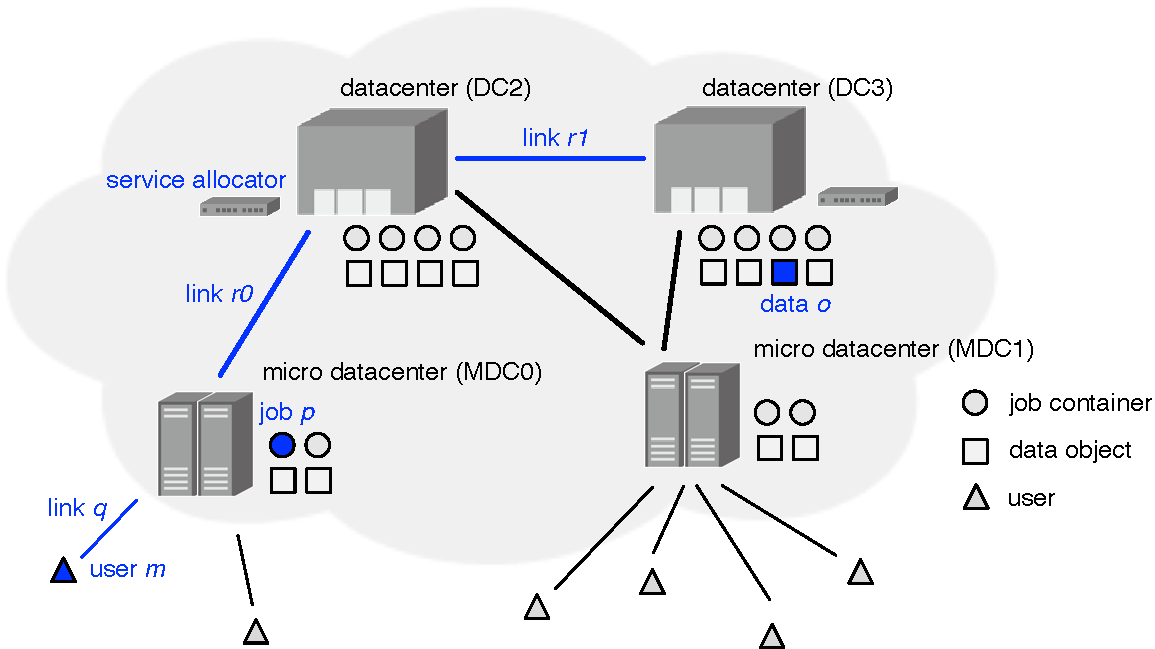
\includegraphics[width=0.825\columnwidth]{figure1-system.pdf}
    \vspace{-1.0ex}
    \caption{Simple system model for job assignment}
    \Description{A simple system model with 2 datacenters and 2 micro datacenters.}
    \label{fig:system}
  \end{center}
\end{figure}

\old{
  Our resource management model is explained using a simple system
  configuration with 2 datacenters (DCs) and 2 micro-datacenters~\cite{Greenberg-2009} (MDCs)
  shown in Figure~\ref{fig:system}.
  When a user requests a service to a nearby service allocation server,
  the service server instantiates the requested service into a series of
  microservice jobs.
  The server obtains the required resource information for each job,
  identifies the locations of the user and the required data object,
  asks nearby resource agents for available resources and their current costs,
  and assigns the job to the node that minimizes the total cost for the
  job.
  The area for cost inquiry could be within proximity along the path
  between the user and the data object.
  The load of a resource can be measured in a number of ways.  Most
  resources have some form of load report functions built-in.
  When the load of a resource fluctuates too rapidly,
  a smoothing filter (e.g., EWMA)
  should be used to stabilize the behavior.
  A load value does not need to be precise, and a rough approximation is
  enough for loose resource management.
  Still, if each allocation is not small enough both in size and in
  duration, the load may not converge as expected.
  Therefore, microservice is the enabler for this approach.
}

\new{
  Our resource management model can be explained through a simplified system configuration consisting of two datacenters (DCs) and two micro-datacenters (MDCs)~\cite{Greenberg-2009}, as depicted in Figure~\ref{fig:system}. When a user initiates a service request to a nearby service allocation server, the server creates a series of microservice jobs to fulfill the request. The server obtains the necessary resource information for each job, identifies the locations of the user and the required data object, and asks nearby resource agents for available resources and their current costs. The job is then allocated to the node that minimizes the overall cost for the service.
  The area for cost inquiry could be within proximity along the path between the user and the data object.
  The load of a resource can be measured in various ways, and most resources have built-in load report functions. If the load of a resource fluctuates too fast, a smoothing filter (e.g., EWMA) should be used to stabilize the behavior. A precise load value is not necessary and a rough estimate suffices for loose resource management. Still, if the allocation is not sufficiently small in both size and duration, the load may not converge as expected. Therefore, microservice is a key enabler for our approach.
}

\subsection{Micro-job Assignment}

\old{
  In this paper, we use a simple micro-job model that defines the
  required resources for a micro-job as $J(p, q, r, s)$ where
  $p$ is the number of micro containers for computation,
  $q$ is frontend communication with the user,
  $r$ is backend communication with data objects (e.g., database), and
  $s$ is the number of time slots.
  The communication costs $q$ and $r$ are also a function of distance so
  that an interactive job with $q \gg r$ will be placed close to the
  user and a data-intensive jobs with $q \ll r$ will be placed close to
  the data.
  For simplicity, we do not distinguish directions of
  communications for $q$ and $r$, and assume only one user and one data
  object per micro-job in this paper.

  A micro-job is specified by a service provider, optionally associated with
  weights, e.g., a service provider may raise the weight for the
  frontend communication to place the job close to the user.
  In this manner, cloud service providers can specify which
  type of resources have priority for a specific service.

  To instantiate a micro-job requested from a user, the service
  server finds the best node to allocate the required resource
  for $J$: $p$, $q$ and $r$ for duration $s$.
  The pseudo cost $E$ to host micro-job $j$ for a unit time at node $i$ for
  user $m$ and data object $o$ is \(E(j, i)     = H(j,i) + G(j,i,m,o)\) where $H(j, i)$ is the computing cost to run $j$ at $i$, and
  $G(j, i, m, o)$ is the communication cost to run $j$ at $i$
  between $m$ and $o$.
  \begin{eqnarray*}
    &&  H(j,i)      = p \cdot f(\rho_{i}) \\
    &&  G(j,i,m,o)  = q \cdot \smashoperator{\sum_{l \in path(m,i)}} f(\rho_{l}) + r \cdot \smashoperator{\sum_{l \in path(i,o)}} f(\rho_{l})
  \end{eqnarray*}
  $f(\rho)$ is the cost function of a resource load $\rho$, and $path(m,i)$ is a set
  of links from $m$ to $i$ (e.g., the shortest path weighted by cost).
  To assign micro-job $j$, the server simply finds the node that minimizes the
  cost: \(argmin_{i} \: E(j, i)\).
}

\new{
  In this paper, we employ a simple micro-job model that defines the required resources for a micro-job as $J(p, q, r, s)$. Here, $p$ denotes the number of micro containers for computation, $q$ denotes frontend communication with the user, $r$ denotes backend communication with data objects (such as databases), and $s$ is the number of time slots. The communication costs $q$ and $r$ are distance-dependent so that an interactive job having $q \gg r$ will be placed close to the user, and a data-intensive job with $q \ll r$ will be placed closer to the data. For the sake of simplicity, we do not differentiate the directions of communication for $q$ and $r$, and assume only one user and one data object per micro-job in this paper.

  A micro-job is specified by a service provider, who can optionally associate weights with it. For instance, a service provider may assign a higher weight to frontend communication to ensure the job is placed close to the user. In this manner, cloud service providers can prioritize which type of resources should be used for a specific service.

  To instantiate a micro-job requested by a user, the service server identifies the optimal node to allocate the required resources for $J$: $p$, $q$, and $r$ for a duration $s$. The pseudo cost $E$ to host micro-job $j$ for a unit of time at node $i$ for user $m$ and data object $o$ is calculated as follows: $E(j, i) = H(j, i) + G(j, i, m, o)$, where $H(j, i)$ represents the computing cost to run $j$ at $i$, and $G(j, i, m, o)$ denotes the communication cost to run $j$ at $i$ between $m$ and $o$.

  \begin{eqnarray*}
    && H(j,i)      = p \cdot f(\rho_{i}) \\
    && G(j,i,m,o)  = q \cdot \smashoperator{\sum_{l \in path(m,i)}} f(\rho_{l}) + r \cdot \smashoperator{\sum_{l \in path(i,o)}} f(\rho_{l})
  \end{eqnarray*}
  $f(\rho)$ is the cost function of a resource load $\rho$, and $path(m,i)$ is a set
  of links from $m$ to $i$ (e.g., the shortest path weighted by cost). To assign micro-job $j$, the server selects the node that minimizes the cost, as expressed by $argmin_{i} : E(j, i)$.
}

\subsection{Pseudo Cost Functions}

%% idea: mechanics model instead of optimization

Our model employs a parametric representation of pseudo cost, as a
function of load, and uses it for load control and also as
backpressure against congestion.
Micro-jobs are naturally gravitated to the most cost-efficient
location.

%% model: cost function: congestion pricing combined with idle-resource pooling
The proposed model is based on congestion pricing in which the cost of
a resource dynamically changes according to the load of the resource.
It works as a barrier function for optimization; the capacity
constraint is enforced by a penalizing cost when approaching the full
capacity.

Another key idea is {\bf idle-resource pooling} that tries to put resources
into an idle state for energy saving.
We propose a convex cost function that enables idle-resource pooling
as part of the congestion pricing mechanism.

A pseudo cost function in our model maps the load of a resource
$\rho \in [0, 1]$ to the corresponding cost.
The capacity limit is enforced by the cost function that rapidly grows
as the load approaches $1.0$, which is known as a barrier function in
optimization theory.

We use two types of pseudo cost functions: one is the monotonic cost
function and the other is the convex cost function.
The monotonic cost function is a simple barrier function that
monotonically grows with load, up to infinity as $\rho \to 1$.
The convex cost function is also a barrier function but also for
idle-resource pooling.
We use the convex form for computing but the monotonic form
for network links as energy-saving-by-idling is not common for
network links.

The standard forms that have the minimum cost of $1.0$ are
shown as bold lines in Figure~\ref{fig:std_costfunc}. We will show how
to manipulate the cost functions in Sec.~\ref{sec:variation}.

\begin{figure}[tb]
  \begin{center}
    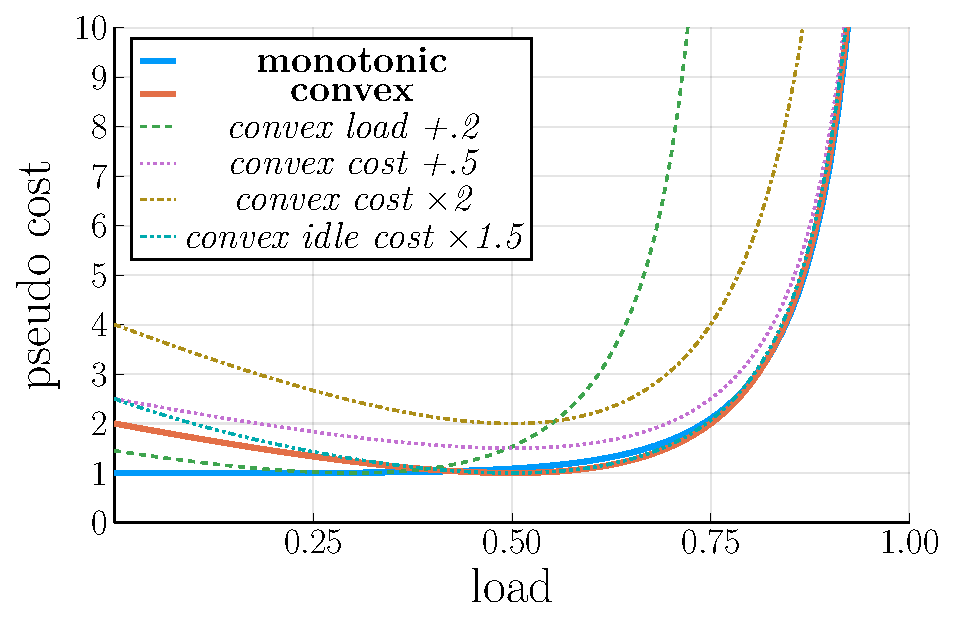
\includegraphics[width=0.9\columnwidth]{figure2-pseudo_costs.pdf}
    \vspace{-2.0ex}
    \caption{Standard cost functions and variants}
    \Description{The standard convex cost function and standard
      monotonic cost function.}
    \label{fig:std_costfunc}
  \end{center}
\end{figure}

The standard convex cost function is defined as:
$f(\rho) = (2\rho - 1)^{2}/(1 - \rho) + 1$.
This function has the properties:
$min\: f(\rho) = f(.5) = 1$, and $f(0) = f(.75) = 2$.
The cost grows rapidly when $\rho > .75$.
The system automatically tries to keep $\rho \le .75$,
aiming at $\rho = .5$.
The standard monotonic cost function is defined as
\( f(\rho) = \rho^{4.5}/(1 - \rho) + 1\)
to roughly match the standard convex cost function in $[.5, .75]$,
the {\em working load range} explained in the next subsection.
Note that the standard forms are defined for convenience, and
other functions with a similar shape also work for our purposes.

\subsection{Idle-Resource Pooling in Action}

The behavior of idle-resource pooling by the convex cost function is
illustrated by the following example in Figure~\ref{fig:4node}.

First, assume a pool of 4 equivalent resources with the standard convex
cost function.
Also, assume that micro-jobs are continuously assigned to the
system; each micro-job is much smaller than the capacity of a
resource.
The initial system load $\sum \rho$ is $0$, and gradually increased up
to $3.5$ until time 350. After time 450, the system load is gradually
decreased back to $0$ until time 800.
Here, load $1.0$ is the capacity of a single resource.
Initially, all resources in the pool are idle, and their costs are
all $f(0)= 2$.
For the first job, one resource $r_{0}$ is randomly selected for allocation, and its
cost becomes lower: $f(0+) < 2$. As a result, subsequent jobs are
assigned to $r_{0}$, with lowering cost towards $\rho = .5$ and then
rising again until $\rho = .75$ where $f(.75) = 2 = f(0)$.
At this point, another resource $r_{1}$ is selected for allocation.
$r_{1}$ is preferred over $r_{0}$ as its cost becomes lower with new
allocations so that both loads move towards $\rho_{0} = \rho_{1} = .5$,
where both are balanced.
Both loads rise again until $\rho_{r0} = \rho_{r1} = .75$,
where the third resource $r_{2}$ kicks in.
It repeats for $r_{3}$, but no more idle resource is available
when $\sum \rho$ reaches $3.0$ so that the loads grow beyond $.75$
up to $\rho = .875$ and $\sum \rho = 3.5$.

When the system load decreases, the process is reversed.
After reaching $\rho = .5$ for all,
one resource with the lowest load $\rho < .5$ becomes more expensive
than the others.
This one is less preferred for subsequent assignments, and quickly
loses the load until it becomes idle again, while the other 3 keep
$\rho$ in $[.5, .75]$. It repeats for the remaining ones.

\begin{figure}[tb]
  \begin{center}
    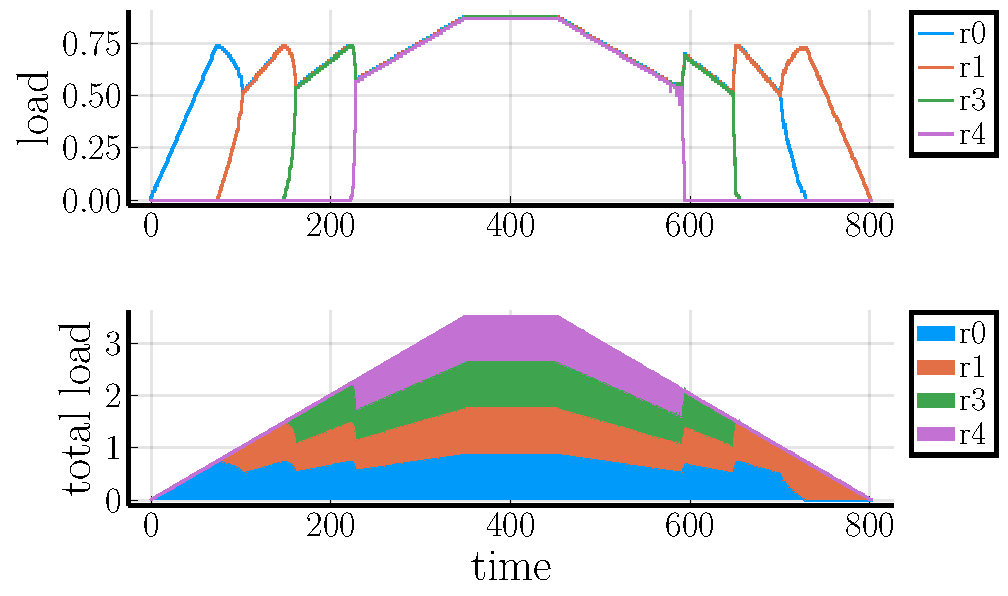
\includegraphics[width=1.0\columnwidth]{figure3-equivalent_nodes.pdf}
    \vspace{-5.0ex}
    \caption{Load distribution among 4 equivalent cost nodes:
      the load of each resource (top) and the total load (bottom)}
    \Description{Simulation results with 4 nodes with the same cost function.}
    \label{fig:4node}
  \end{center}
  \hspace{0.8\columnsep}
\end{figure}

\begin{figure}
  \begin{center}
    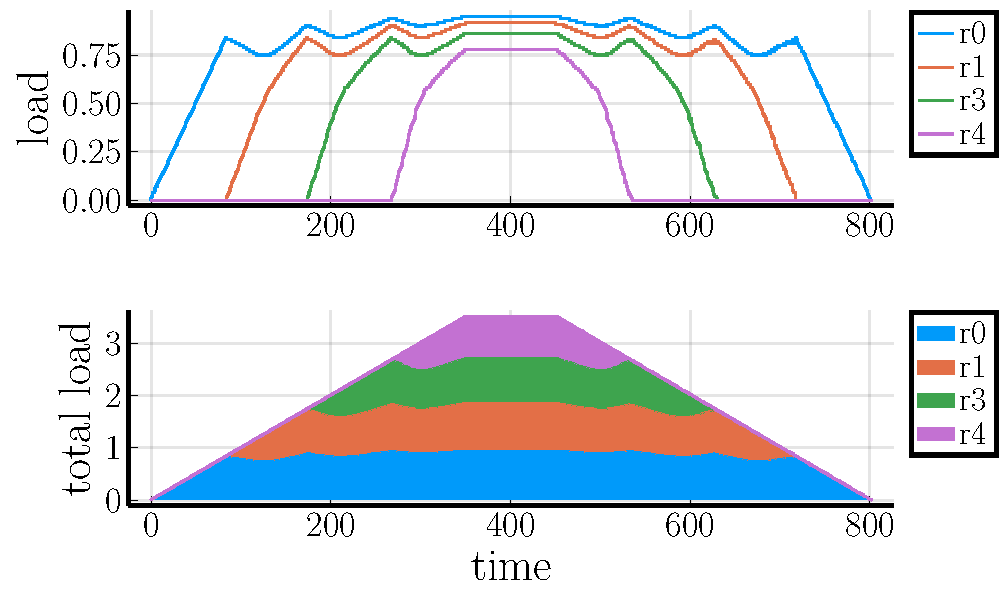
\includegraphics[width=1.0\columnwidth]{figure4-proportional_nodes.pdf}
    \vspace{-5.0ex}
    \caption{Load distribution: 4 proportional cost nodes}
    \Description{Simulation results with 4 nodes with proportional cost function}
    \label{fig:4node-ratio}
  \end{center}
\end{figure}

It is easy to see how the number of active resources changes when
there are more resources.
When the number of active resources is increasing, the load of each
active resource stays at around $\rho = .75$.
On the other hand, when the number of active resources is decreasing,
the load of each active resource stays at around $\rho = .5$.
In short, when all resources are equal, the system tries to maintain
the load of active resources in the {\em working load range}
$[.5, .75]$, while keeping idle resources as much as possible.

The usage of a resource can be controlled by manipulating the cost
function.
%When resources are not equal, the behavior becomes more complex, but
%the underlying mechanisms are the same.
Let's change the costs of the 4 resources with the ratio $1:2:4:8$,
that is $8 f_{r0} = 4 f_{r1} = 2 f_{r2} = f_{r3}$.
Figure~\ref{fig:4node-ratio} shows the load distribution.
Here, we focus on the interaction between $r_{0}$ and $r_{1}$ since
the other interactions are similar.
To activate $r_{1}$, the load of $r_{0}$ goes up to $.84$ to satisfy:
$f_{r1}(0) = 4 = f_{r0}(.84)$.
When $r_{1}$ is moving towards idle after time 700, the load
of $r_{0}$ is $.75$ to satisfy: $f_{r1}(.5) = 2 = f_{r0}(.75)$

For unequal resources in general, the required load to trigger a new
allocation is higher than $\rho = .75$ for the already
active ones to match the cost $f(0)$ for the new one, but the load
will not go much further as the slope of the cost function is steep.
Similarly, when the most expensive one among active resources becomes
idle, the load of the remaining ones stay at the matching cost
$f(.5)$ for the deactivating one.

%%Note that our goal is not to achieve the theoretical optimum but to
%%enable loose automatic distributed load balancing.

\subsection{Manipulating the Cost Function}
\label{sec:variation}

The utilization of a resource can be manipulated by modifying the cost
function of the resource as shown as the variants in Figure~\ref{fig:std_costfunc}.
One can {\em lower or raise the load level} of a resource by shifting
the load in the cost function and adjusting the target load,
$f'(\rho) = f(\rho + \Delta)$.
To {\em change the activation order} in the idle-resource pooling,
one can raise or lower the cost,
e.g., by making the cost  $n$ times more expensive, $f'(\rho) = n f(\rho)$.
For minor adjustment, one can use an additive form,
$f'(\rho) = f(\rho) + \Delta$.
To make {\em idle-resource pooling more aggressive},
one can raise the cost at $\rho = 0$:
e.g., to raise the cost at $\rho = 0$ by a factor of $(n+1)/2$,
$f'(\rho) = n (2\rho - 1)^{2}/(1 - \rho^{n}) + 1$.

A {\em premium service} can be realized by shifting the load
in the same way as lowering the load level
but for specific users or jobs (not for a specific resource) so as to
have premium jobs always being assigned to less loaded resources.
Similarly, an {\em economy service} that allows to be assigned to more
loaded resources can be made by a negative shift.
It would be appealing as a business model to enable multiple classes using a single
resource pool with a single shift parameter.

% \begin{figure}[tb]
%   \begin{center}
%     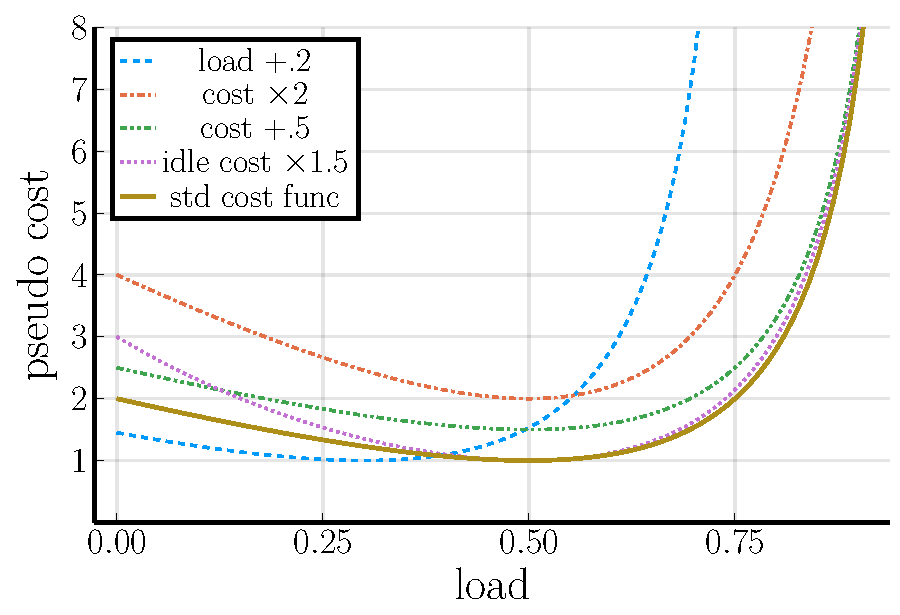
\includegraphics[width=0.9\columnwidth]{figure5-custom_pseudo_costs.pdf}
%     \vspace{-2.0ex}
%     \caption{Manipulating convex cost functions}
%     \Description{Variations of manipulated cost functions are shown.}
%     \label{fig:costfunc3}
%   \end{center}
% \end{figure}

Other than manipulating the cost function,
cloud service providers can adjust the required resources and their
weights for a job.  Also, it is effective to place data objects close to the
users, and both service providers and their users should have some
control over where to store the data.
Thus, the system allows stakeholders to loosely control the
resource utilization.
